\section{OpenCL}

\subsection{What is OpenCL?}
OpenCL is specified by the Khronos Group in the OpenCL 1.2 Specification as follows:

\begin{quotation}
OpenCL (Open Computing Language) is an open royalty-free standard for general purpose
parallel programming across CPUs, GPUs and other processors, giving software developers
portable and efficient access to the power of these heterogeneous processing platforms. \cite{opencl_spec}
\end{quotation}

The Khronos Group is an industry consortium who maintains OpenCL as an open standard. This means that the Khronos Group offers a specification of the OpenCL API and a detailed description about its functionality and behavior for free. This specification can be downloaded at their website \cite{opencl_spec}. Maintaining the OpenCL standard consequently means, that the Khronos Group neither provides software development kits (SDKs), drivers that implement OpenCL nor hardware that it can make use of. These concerns are subject to other companies called vendors, which are typically hardware manufacturers providing necessary developing resources and include OpenCL support in their drivers. Examples of such companies are the two famous graphic card vendors NVIDIA and AMD as well as the renowned processor manufacturer Intel.

Unlike other famous APIs the Khronos Groups specifies that are very specific in their usage or the targeted hardware (like the famous 3D API OpenGL used to drive graphic hardware), OpenCL is a general purpose programming framework. It was conceived with universality in mind offering almost no restrictions on the field of application it may be used. Portability from its well designed hardware abstraction model which enables it to run on many different kinds of devices, even ones which may have not been created yet, is one of OpenCL most powerful strengths. Such devices may be classical CPUs and GPUs, but also more uncommon types of hardware like FPGAs (field programmable gate arrays), DSPs (digital signal processors) or Intel's MICs (Many Integrated Core) \cite{mic}. Moreover, OpenCL may be used to combine multiple available devices into a single heterogeneous platform extending an applications processing resources beyond the bounds of individual pieces of hardware.

Additionally to being independent of a specific purpose and decoupled from the underlying hardware, OpenCL is also available across all mayor operations systems including Windows, Linux and Mac OS X.

With the upcoming specification of WebCL currently only available as a working draft, OpenCL will eventually even find its way into web browsers and the HTML5 technology conglomeration. Thus making it even independent of an operating system and bringing high performance computing into web applications.

\subsection{Components}

OpenCL is not an API alone. As it allows programs to run on hardware that may have certain restrictions or offer different features than a classical CPU, traditional languages like C++, Java or C\# can not be used to write those programs. Therefore, the OpenCL standard includes the specification of a separate language that is used to write small programs that are executed on a hardware device. These programs are called kernels and are written in the OpenCL C language, which is a restricted version of C99 with extensions for vectorization and handling OpenCL's abstract memory model.

The allow OpenCL to support many different hardware platforms it consists of the following components:

\begin{description}
	\item[API] \hfill \\
	The application programming interface is specified by the Khronos Group ensuring that every vendor implementation of OpenCL is compatible and exchangeable. The API is provided as a set of a C header files that a software developer can download from Khronos' website. These headers are typically also shipped within an SDK. Khronos additionally specifies a C++ wrapper for the C API. Bindings for other language exists but are not maintained by Khronos.
	The API is used by a conventional program (e.g. written in C++) to run kernels on an OpenCL capable device. This program is called the host application.
	\item[SDK] \hfill \\
	The software developing kit is the main collection of tools and resources a software developer needs to write applications using OpenCL. An SDK is usually provided by a vendor, an implementor of OpenCL. Examples of such SDKs are the NVIDIA CUDA Toolkit and AMD's Accelerated Parallel Processing (APP) SDK. These SDKs typically contain header files to be included by a C/C++ program and static libraries for the C/C++ linker which are responsible for binding to the OpenCL driver at runtime. Furthermore, code examples, tutorials, documentation, developing tools etc. may be additionally provided depending on the vendor. With headers and static libraries an SDK contains all resources necessary to write and compile an OpenCL application.
	\item[OpenCL C language] \hfill \\
	Kernels are typically written in separate source files using the OpenCL C language. An OpenCL application reads these source files at run time and sends them to the OpenCL compiler to create a binary for one or more available hardware devices where it may be executed. A source file written in the OpenCL C language may consist of several functions, variable definitions, control flow statements, comments, etc. but has to have at least one function prefixed with the \_\_kernel attribute, which may be called by the host application through the OpenCL API and serves as an entry point into a kernel.
	\item[OpenCL C Compiler] \hfill \\
	OpenCL kernels must be compiled for a specific platform before they can be executed. This compilation process is initiated and controlled by the host application through the API. This separate compilation at run time is required to retain OpenCL's portability as an OpenCL application may be deployed on any kind of machine with a suitable driver. As a result the available OpenCL implementation (providing the compiler) and the used hardware device (affecting the compiler's output) may only be determined at runtime.
	\item[Driver] \hfill \\
	Finally, the driver is OpenCL's core. It implements the OpenCL API and maps the functionality specified in the standard to a vendor's hardware. The host application uses the driver through the API to initialize OpenCL, compile kernels, allocate memory resources, initiate computations and communicate with kernels running on a device. A driver is always specific to a dedicated hardware and must therefore be provided by a vendor. The driver is sometimes also referred to as Installable Client Driver (ICD).
\end{description}

\subsection{Hardware architectures}

One of the greatest advantages of OpenCL and also one of the biggest influences on its design is OpenCL's ability to support devices of many different hardware architectures. These devices can be used through OpenCL by the same common API and may even be used together in a single application or computation, which is sometimes referred to as heterogeneous computing.
A closer look into the architectures of the two most common hardware devices, namely a CPU and a GPU, may aid the reader to better understand design decisions made by the Khronos Group when OpenCL was conceived. Furthermore, a deeper understanding of graphics hardware will be needed for the implementation chapters of this thesis.

\subsubsection{The Central Processing Unit (CPU)}

\begin{figure}[h] % http://www.bakesi.com/2012/12/intel-core-processors-may-soon-get-less.html and cache hierarchy: http://hothardware.com/Reviews/Intel-Core-i7-Mobile-Processor-Launch-Review/?page=2
\centering
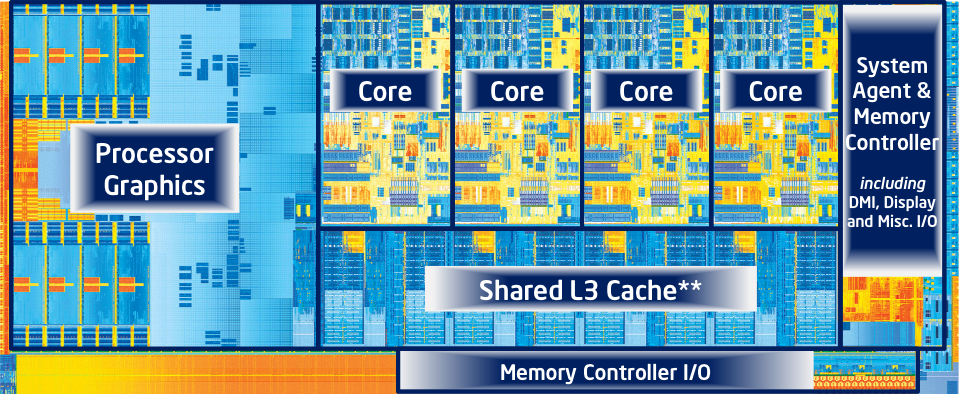
\includegraphics[width=0.9\linewidth]{ivy_bridge}
\caption{Architectural overview of an Intel Ivy Bridge Processor \cite{}}
\label{fig:ivy_bridge}
\end{figure}

The CPU is the kind of processors developers are mostly used to. Software written in common languages like C++, Java or C\# is directly or indirectly (using a Virtual Machine) executed on this kind of hardware.
In figure \ref{fig:ivy_bridge} we can see the design of a modern processor by the example of an Intel Ivy Bridge quad-core. One can clearly see the four physical cores of the processor. Thanks to hardware multithreading (Hyper-threading in Intel terms) each physical core can process a pair of threads which are seen as two virtual CPUs by the operation system resulting in 8 available cores for an application.
Note the on-chip graphics processor in the Ivy Bridge architecture which can be used as a replacement for a graphics card but is not used as general processing device such as the CPU's cores.

When it comes down to calculative throughput and the problem offers some degree of data parallelism (several chunks of data are processed equally), SIMD (Single Instruction Multiple Data) features of the CPU can be used to multiply the number of input elements an instruction can process. Intel's Ivy Bridge for example allows the parallel execution (vectorization) of up to four (SSE4 - Streaming SIMD Extensions 4) or eight (AVX - Advanced Vector Extensions) single precision floating point operations.

Considering memory access, the CPU uses the standard data bus to communicate with the external main memory. As this communication usually takes a while (up to hundreds or even thousands of CPU cycles  \cite[p. 54]{opencl_book}) the CPU uses a hierarchical cache system. Each core has it's own level one and level two cache, which have to be kept synchronized. All cores share a common level three cache that is then connected to the memory controller.

From a performance concerned developer's perspective, all we have to pay attention to is to have enough parallelism in our application to utilize all cores of our CPU (which is a number around 2, 4, or 8). If our application has to process large amounts of data using the same operations on elements of the input (e.g. multimedia applications like image or video processing), vector instructions may be used to speed up execution. Regarding memory, beside small tips to improve cache effects the developer has only limited power to optimize, as the entire cache system is controlled by the CPU and operation system. 


\subsubsection{The Graphics Processing Unit (GPU)}

When we think of a GPU we think of a highly parallel graphics orientated processing device.

From its introduction with OpenCL in 1989 till the creation of the first GPGPU languages in 2004 (See section \ref{sec:history} for more details about the history of GPUs) the architecture of a GPU's hardware followed the principles of the graphics pipeline. Therefore, GPUs developed from original desktop processors to (as written in \cite{opencl_book}) heavily multithreaded devices employing sophisticated task management directly in hardware. This was needed to cope with complex task graphs processing vertices, geometry and pixels. This tasks and the data they process are highly parallel representing an extensive amount of independent work which is therefore most suitably handled by a device with a great amount of cores employing latency tolerant multithreading \footnote{Latency tolerant means that the hardware is insensitive to longer lasting memory requests.}.

\begin{figure}
\centering
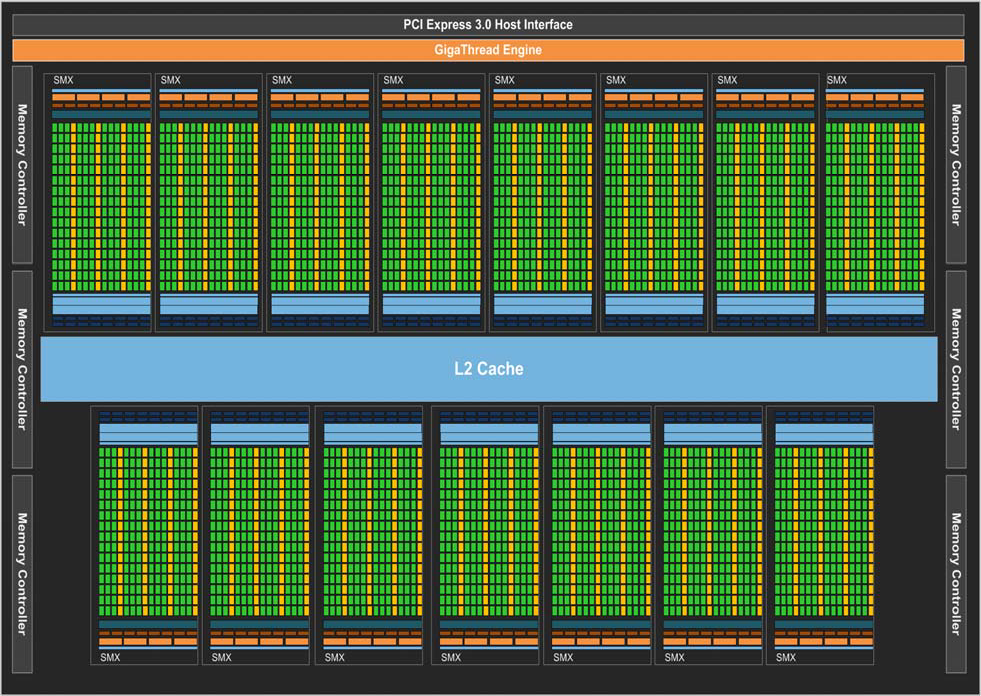
\includegraphics[width=0.9\linewidth]{kepler_arch}
\caption{Full chip block diagram of NVIDIA's Kepler GK110 architecture containing 15 Streaming Multiprocessors (SMX) \cite{kepler_arch}.}
\label{fig:kepler_arch}
\end{figure}

\begin{figure}
\centering
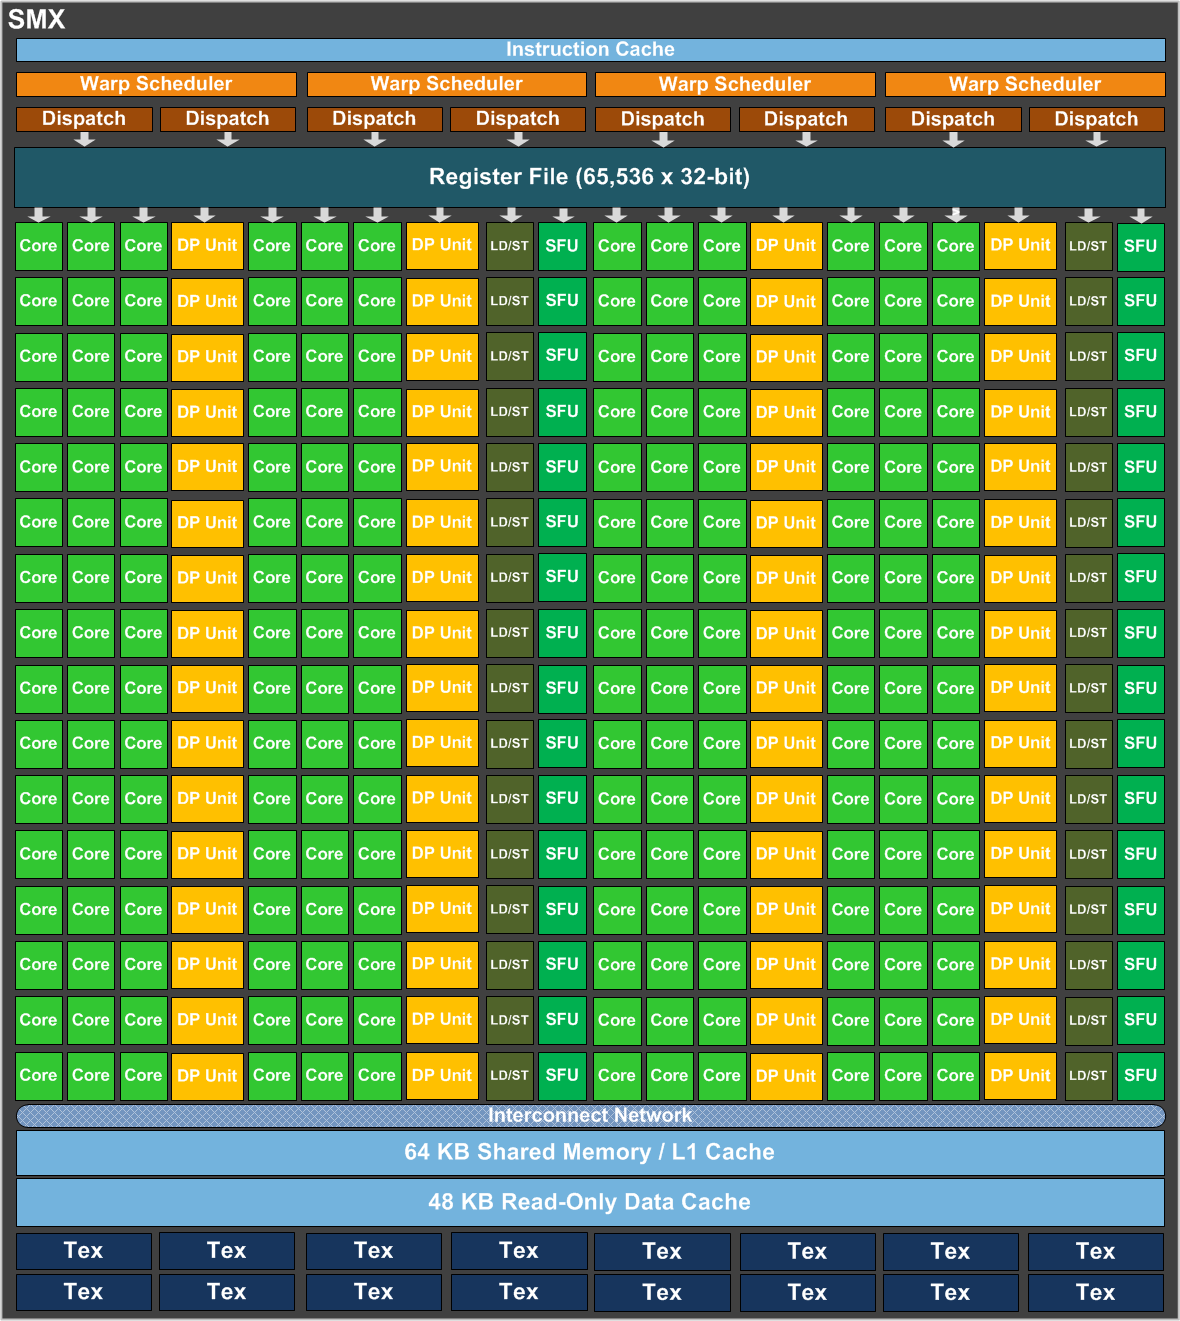
\includegraphics[width=0.9\linewidth]{kepler_arch_smx}
\caption{Architecture of a Streaming Multiprocessor (SMX) of NVIDIA's Kepler GK110 architecture containing 192 single precision CUDA cores, 64 double precision units, 32 special function units (SFU), and 32 load/store units (LD/ST) \cite{kepler_arch}.}
\label{fig:kepler_arch_smx}
\end{figure}

In figure \ref{fig:kepler_arch} we can see the design of a modern GPU by the example of NVIDIA's Kepler architecture. On the top side of the block diagram the PCI Express controller is placed. This interface is responsible for the communication of the graphics card with the CPU through the mainboard's PCI Express bus. After data has arrived at the graphics device, it has to be scheduled for processing to one or more of the streaming multiprocessors (SM, or SMX in NVIDIA's Kepler architecture terms). A SM is not a core but more an aggregation of many cores with additional scheduling logic and therefore representing an extra hierarchical step in a GPU's workflow. This is one of the first bigger differences in the architecture of modern GPUs when compared with traditional CPUs.

Figure \ref{fig:kepler_arch_smx} shows a detailed view of the structure of a streaming multiprocessors. Once a package of data is scheduled to a SM, it is then prepared for execution by the Warp Schedulers. A Warp (or Wavefront in AMD terms) is a block of threads (32 in NVIDIA's Kepler architecture) executing the same instructions in parallel along cores managed by the Warp Scheduler. This concept is often called SIMT (Single Instruction Multiple Threads). The difference to SIMD (Single Instruction Multiple Data) is that SIMD requires a vector instruction in each thread whereas SIMT only uses scalar code. The vectorization is handled by the hardware \cite[p.99]{gpu_optimizations}. A Warp Scheduler is able to manage multiple Warps (up to 64 on the Kepler GK110 architecture \cite[p.7]{kepler_arch}) at the same time which may be executed interleaved on the cores (similar to the two threads in a hyper-threading Intel core). This allows to hide memory latency because when a Warp has to stall because of a memory request, the Warp Scheduler can execute other Warps until the memory request is satisfied.

\begin{figure}
\centering
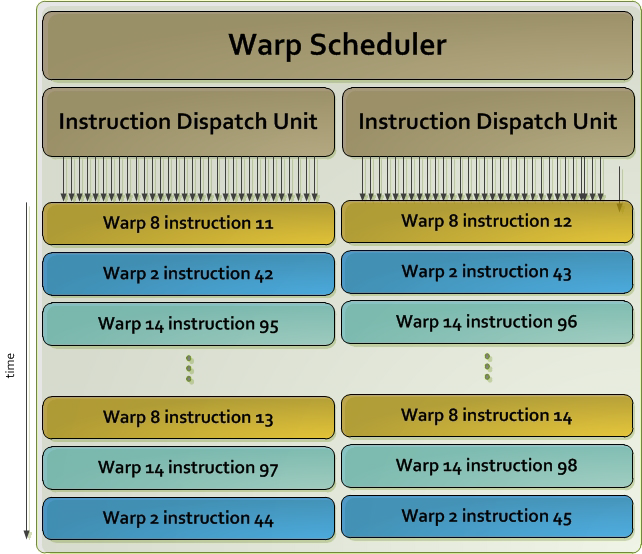
\includegraphics[width=0.9\linewidth]{warp_scheduler}
\caption{Closer look on a Warp Scheduler. Each Warp Scheduler has two dispatcher units allowing the execution of two independent instructions of a Warp in parallel.}
\label{fig:warp_scheduler}
\end{figure}

Another important thing to notice is that all cores within a SM share the same registers. This plays an important role when choosing the right number of Warps to run concurrently on the SM. Too less Warps may result in unused core cycles whereas a too large number of Warps may request more registers than there are available at the SM. The additionally needed registers are then allocated in the slow global memory. This concern will be discussed later in chapter \ref{sec:execution_model}.

The actual work is then performed in the cores itself. The major number of cores (labeled "Core" in green in figure \ref{fig:kepler_arch_smx}) are used for single precision floating point and integer arithmetics. In contrast to older GPUs modern graphics processing units also include support for double precision floating point arithmetic, which was not needed for graphical calculations but becomes increasingly important in GPGPU computing. The Kepler architecture serves this need by a dedicated core (labeled "DP Unit"). Additional hardware resources include the load and store unit for register and memory access and the special function unit (labeled "SFU"). On the bottom of figure \ref{fig:kepler_arch_smx} we find the texture units which are heavily used in 3D graphics. They can also be used by OpenCL as a special kind of memory (more in chapter \ref{sec:matrix_mul}).

Finally, beside the way of executing threads on its cores, the memory system is the second aspect of a GPU that shows significant differences when compared with a CPU. Although also using a hierarchical cache system, the GPU lacks caches for each individual core. The first level cache resides within the SM and is used by all cores inside the SM. A specialty of the GPU is the shared memory (also scratch pad memory or local memory) which can be seen as a programmer controllable cache. An OpenCL kernel may use this small block of memory to cache data from the global memory and to limitedly share data with other threads (more on this in chapter \ref{sec:workgroups}). Outside the SM (figure \ref{fig:kepler_arch}) the GPU offers a larger level two cache which is then connected to multiple memory controllers to access the global memory. The global memory resides on the graphics card outside the GPU (such as the RAM is outside a CPU) and has a larger size of up to one or two GiB. An important difference of the global memory when compared with the RAM on the mainboard is that RAM can be accessed in almost any pattern without significant performance penalties. This is very different for a GPU where memory request should be coalesced \footnote{A coalesced memory access occurs when all threads of a Warp request data on consecutive memory addresses resulting in a fast memory block transfer instead of individual transfers of small chunks.} and blocked across the threads of a warp to achieve optimal memory bus utilization.

Concerning the performance of a GPGPU accelerated application there are a huge amount of concerns to worry about. Two of them have already been discussed, namely choosing the right number of warps concurrently executing on the SMs and paying attention to memory access. For the latter, the memory access pattern should be coalesced and frequently needed or shared data should be cached in shared memory. Further optimizations exist but would exceed the scope of this thesis. For further reading, NVIDIA has a detailed paper on this subject \cite{gpu_optimizations}.

\subsection{API Overview}

OpenCL is specified using the C programming language. The Khronos Group defines a set of C functions, types and constants that make up the API a developer can use to write applications using OpenCL. These declarations are cumulated into the cl.h C header file, which can be downloaded from the website of the Khronos Group and can typically also be found in the include directory of any OpenCL SDK. Although specified in C OpenCL has an object orientated design. The UML class diagram in figure \ref{fig:opencl_uml} shows the objects which can be created, queried and manipulated using corresponding API calls. The Khronos Group also specifies a C++ Wrapper with OpenCL 1.1 built atop the C API which will not be used in this thesis.

The following chapters will give the reader a brief introduction into OpenCL's design and relevant API functions. 

\begin{figure} % from http://http.developer.nvidia.com/CgTutorial/cg_tutorial_chapter01.html
\centering
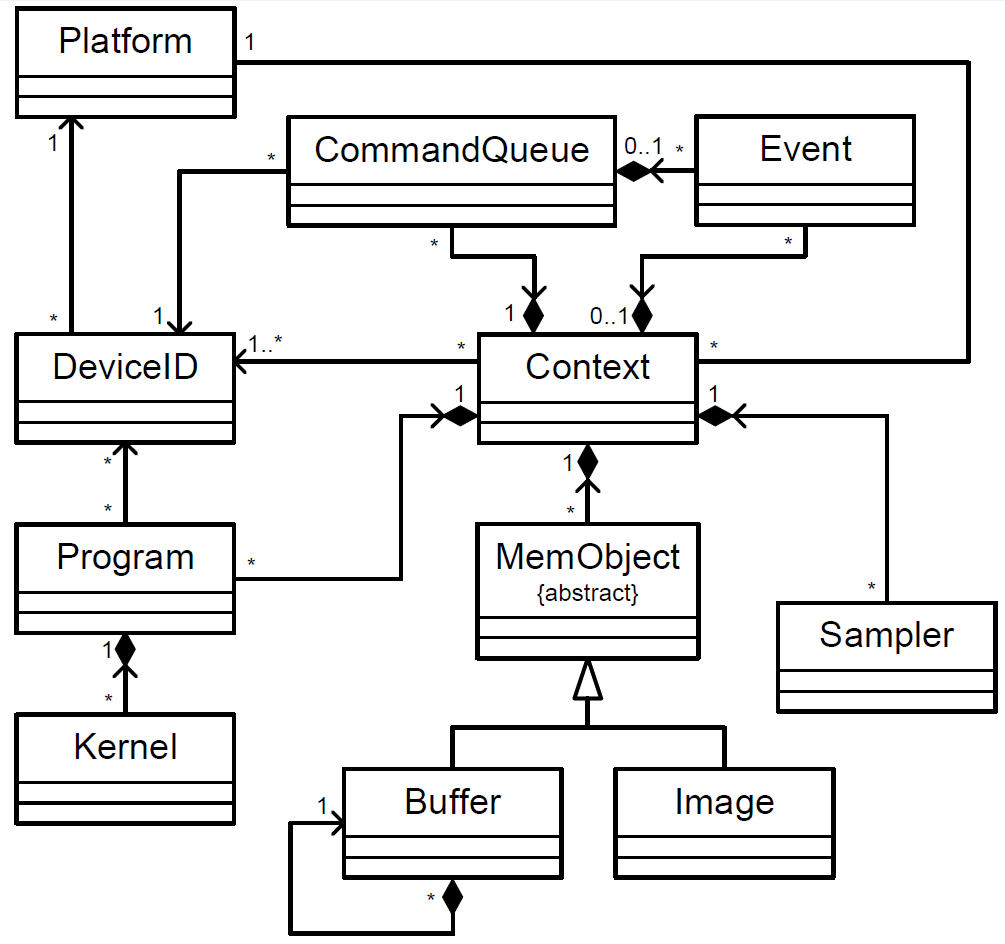
\includegraphics[width=0.9\linewidth]{opencl_uml}
\caption{OpenCL class diagram \cite{opencl_spec}}
\label{fig:opencl_uml}
\end{figure}

\subsection{Platform model}
platforms, devices



\subsection{Execution model}
\label{sec:execution_model}
 command queues, programs, kernels
what is a kernel?

how are kernels executed?
work groups, work items
hardware threads (synchronization)

choosing the right work group size


\subsection{Memory model}
buffers and images

\subsubsection{Types of memory}
different types of memory on the GPU
global local constant private
texture, pinned memory
performance
how do we access them?

\subsubsection{General design considerations}
coalesced memory access
local memory as programmable cache (and method of sync)
bench conflicts

\subsubsection{Data transfer}
read, write buffers
sync, async

